\section{Method}
\label{sec:cvpr_method}

\subsection{Optical flow from contrast maximization}

Each pixel in an event camera independently detects changes in brightness and generates an event $e_k = (t_k, \boldsymbol{x}_k, p_k)$ when this change exceeds a preset threshold. The polarity $p_k \in \{+1, -1\}$ indicates whether the brightness at pixel $\boldsymbol{x}_k$ and time $t_k$ increased or decreased. Contrast maximization~\cite{gallego2018unifying,gallego2019focus} assumes these events $\mathcal{E} = \{e_k\}_{k=1}^{N_e}$ are triggered by motion, meaning that a warp $e_k = (t_k, \boldsymbol{x}_k, p_k) \mapsto e'_k = (t_\text{ref}, \boldsymbol{x}'_k, p_k)$ with the correct motion estimate $\Delta\boldsymbol{x}_k$ will align it with other events triggered by the same portion of a moving edge, increasing the contrast of the image of warped events (IWE).

We follow the contrast maximization framework as in~\cite{paredes-valles2023taming}, which estimates optical flow for thin slices of the event stream using a recurrent architecture. By concatenating flows $\boldsymbol{u}_i$ as $\Delta\boldsymbol{x}_k=\sum_i(\Delta t_i \boldsymbol{u}_i)(e_k)$, events can be warped iteratively to neighboring slices, with the correct flows leading to sharp IWEs at all reference times along the trajectory:
\begin{equation}
    \mathcal{L}_\text{CM} = \frac{1}{T + 1} \sum_{t_\text{ref} = 0}^T \frac{\sum_k \bar{t}_k(t_\text{ref}) \kappa(\boldsymbol{x}_k)}{\sum_k \kappa(\boldsymbol{x}_k)}
    \label{eq:cvpr_multiref}
\end{equation}

where $\bar{t}_k(t_\text{ref})$ is the timestamp contribution of event $e_k$ to the IWE at reference time $t_\text{ref}$, and $\kappa$ is a bilinear splatting kernel. We regularize (prevent event collapse) by scaling IWEs by the number of pixels with at least one event and by masking events that get warped out of the image space at any point~\cite{hagenaars2021selfsupervised,paredes-valles2023taming}.

\subsection{Combining depth and ego-motion into flow}

Assuming a static scene and no occlusion/disocclusion, depth and ego-motion can be accurately estimated from monocular video alone~\cite{zhou2017unsupervised}. The optical flow used to warp a pixel $\boldsymbol{x}$ between different views is constructed from depth $D$ and a camera transformation or relative pose $P$:
\begin{equation}
    \boldsymbol{x}' \sim KPD(\boldsymbol{x})K^{-1}\boldsymbol{x}
\end{equation}

with $K$ the camera intrinsic matrix, $P$ consisting of a rotation $R$ and a translation $\boldsymbol{t}$, and $\sim$ because depth is only defined up to a scale.\footnote{For simplicity, we omit the conversion to homogeneous coordinates.} The network estimates depth $D$ directly using a softplus activation~\cite{gordon2019depth}; relative pose $P$ is estimated with rotation expressed in exponential coordinates $\boldsymbol{\omega}$~\cite{wang2018learning}, and converted to $R$ using Rodrigues' formula.

To encourage consistent scale for consecutive depth predictions, we include the geometry consistency loss from~\cite{bian2019unsupervised}, which computes a normalized difference between the forward-projected depth $D_{0\shortrightarrow1}$ and interpolated depth $D'_1$ for all valid pixels $\boldsymbol{x}\in V$ (visible in both images):
\begin{equation}
    \mathcal{L}_\text{geo} = \frac{1}{\lvert V \rvert} \sum_{\boldsymbol{x}\in V} \frac{\lvert D_{0\shortrightarrow1}(\boldsymbol{x}) - D'_1(\boldsymbol{x}) \rvert}{D_{0\shortrightarrow1}(\boldsymbol{x}) + D'_1(\boldsymbol{x})}
\end{equation}

where we average over the number of valid pixels $\lvert V \rvert$. Setting an appropriate weight $\lambda$, this then results in the full loss formulation as:
\begin{equation}
    \mathcal{L} = \mathcal{L}_\text{CM} + \lambda\mathcal{L}_\text{geo}
\end{equation}

\begin{figure*}
    \centering
    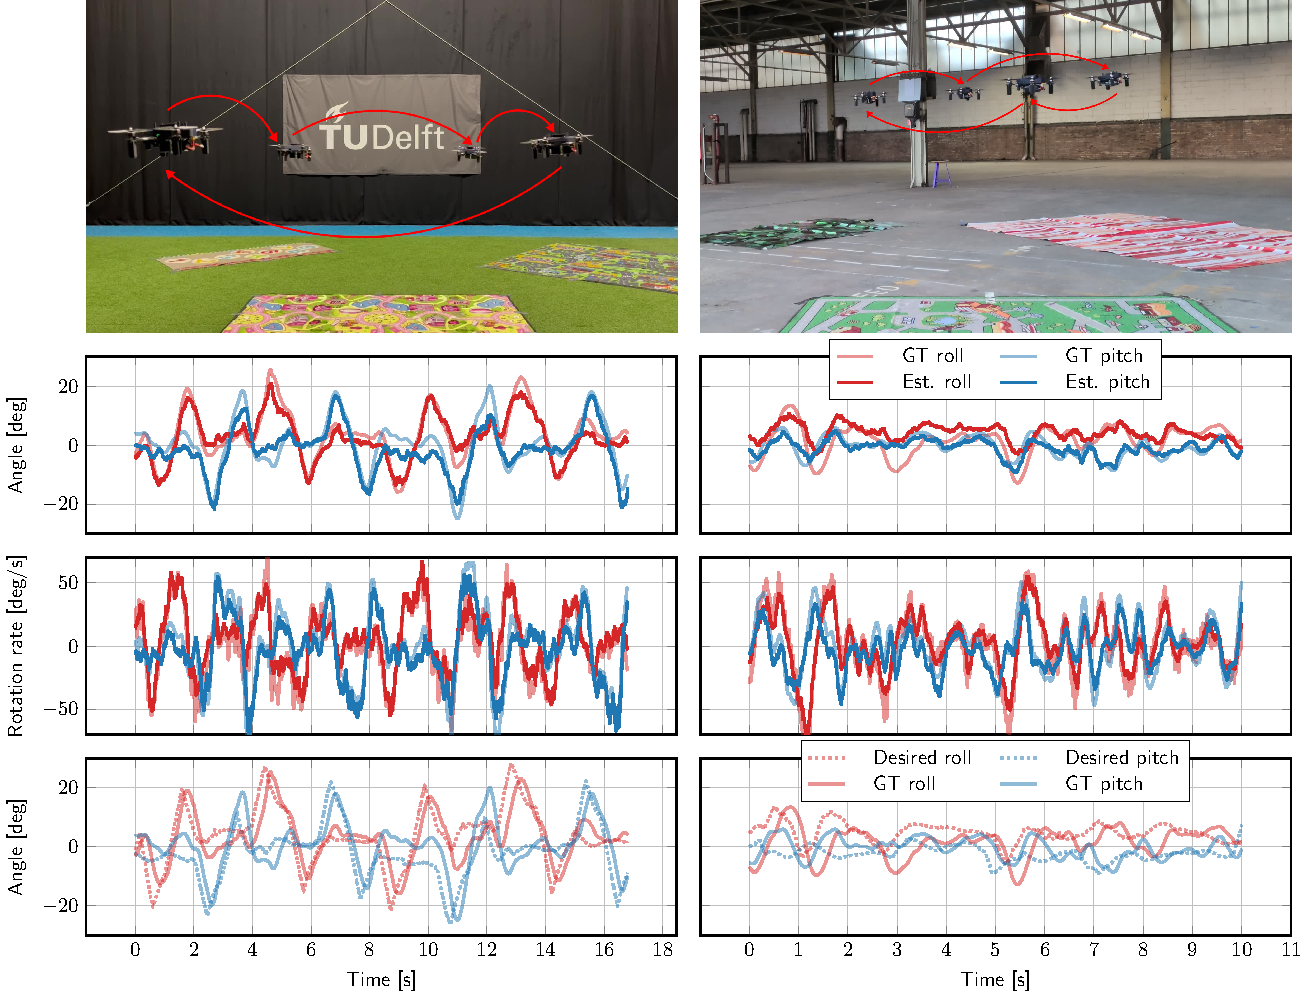
\includegraphics[width=\linewidth]{04_chapters/CVPR25/cc_figures/tikz-figure1.pdf}
    \caption{\textbf{Top left:} events $e$ of different polarities are warped forward and backward by bilinearly sampled (BS) optical flows $\boldsymbol{u}$. Events warped outside the image are discarded. Next, events are bilinearly splatted to IWEs (images of warped events) at all reference times $t^*_\text{ref}$. \textbf{Bottom left:} batched processing of events such as in~\cite{paredes-valles2023taming} requires zero-padding bins of events to equal length to facilitate simultaneous warping to neighboring reference times. In contrast, our per-event parallel processing in CUDA warps all events independently, doing away with padding and allowing to warp only those events still in the image space. \textbf{Right:} Runtime and peak increase in memory consumption for different phases of computing the contrast maximization loss on an NVIDIA RTX 4090 and Jetson Orin NX. 10\% of each bin is made up of padding, which is not processed by the CUDA implementation. We indicate the range of events per bin for common datasets~\cite{delmerico2019are,zhu2018multivehicle} in black. Naive PyTorch processes all events in a for-loop. While batching events together improves a lot over this, parallel processing of all events in CUDA results in even bigger speedups with less memory consumed.}
    \label{fig:cvpr_cuda}
\end{figure*}

\subsection{Optimizations for on-device learning}

For efficient prediction, we make use of a lightweight, 430k-parameter network inspired by~\cite{wu2024lightweight}. It consists of a strided convolutional encoder, a ConvGRU recurrent bottleneck, and a two-tailed convolutional decoder for depth and ego-motion (more details in the supplementary material). While one network forward pass takes less than a millisecond on an NVIDIA RTX 4090, computing the contrast maximization loss and backpropagating the resulting gradients each take up more than 10~ms.

To make on-device learning feasible, we have to improve the efficiency of the components that make up the loss computation and network update: i) warping all events in the accumulated set of events $\mathcal{E}$ using a sampled optical flow to all reference times $t_\text{ref}\in [0, T]$, ii) bilinearly splatting them to the IWE at that $t_\text{ref}$, iii) computing the gradient with respect to the network parameters.

Previous work~\cite{paredes-valles2023taming} warped and splatted events in batches using PyTorch functions. This has multiple inefficiencies. Batching different amounts of events together leads to padding with zeros, resulting in wasteful computation and memory usage. This also goes for warping events that already went out of the image space (and therefore do not contribute to the loss anymore). Furthermore, some operations (like bilinear splatting) do not have optimized implementations in PyTorch. All this combined results in extra computational and memory overhead due to intermediate tensor allocations, multiple instead of single kernels, computation graph tracking and scattered memory accesses.

The abovementioned issues can be resolved by considering that all events independently contribute to the loss since they are summed in the IWEs, and that we can therefore parallelize over all the accumulated events $\mathcal{E}$. We implement the functions to do so in CUDA, getting rid of most of the overhead, and connect them to PyTorch as an extension. 

Specifically, we assign one CUDA thread to handle one or more events in parallel, read off their positions in the 3D domain $(x,y,t)$, and then apply the flow fields to ``push'' each event through time either forward or backward in an iterative fashion. During the backward pass, we use the stored warped-point positions along each time step (forward and backward) to compute partial derivatives w.r.t the flow vector $\frac{\partial \mathcal{L}}{\partial \mathbf{f}}$. As in the forward pass, we rely on bilinear interpolation weights at each $(x,y)$ to distribute gradients to the four nearest flow-vector cells. By avoiding padding and unnecessary warping computations, we achieve significantly better parallelization on GPUs.

As shown in \cref{fig:cvpr_cuda}, the resulting improvements are, depending on the device, roughly 100x in terms of runtime, and 2-5x in terms of memory consumption. Common datasets like UZH-FPV~\cite{delmerico2019are} and MVSEC~\cite{zhu2018multivehicle} have between 1k and 10k events per bin, well within the range of these speedups. Furthermore, looking at the peak delta memory, the removal of padding yields much lower memory consumption when event data is highly sparse. Because we now provide the analytical gradients in the CUDA backward kernel, these do not have to be computed through automatic differentiation, leading to further efficiency improvements.

\subsection{Using depth for obstacle avoidance}

In the absence of metric depth and with a possibly varying scale, we can construct simple obstacle-avoiding behaviour using the difference in predicted depths for different parts of the field-of-view~\cite{liu2023nano,chakravarty2017cnnbased}. More specifically, we slice the depth map into $K$ vertical bins, compute the average inverse depth $d_k$ for each, and use these to set a desired yaw rate $\dot{\psi}$:
\begin{align}
    \dot{\psi} &= \dot{\psi}_\text{goal}(\boldsymbol{d}) + \dot{\psi}_\text{avoid}(\boldsymbol{d}) \\
    \dot{\psi}_\text{goal}(\boldsymbol{d}) &= \lambda_\text{goal} (\argmin_k (d_k) - \bar{k}) \\
    \dot{\psi}_\text{avoid}(\boldsymbol{d}) &= \lambda_\text{avoid} \sum_{k=0}^{K-1} (\bar{k} - k) e^{(-\frac{\alpha}{d_k})}e^{(-\frac{(k - \bar{k})^2}{2\sigma^2})}
\end{align}

where yawing to the right is positive, and $\bar{k}=\frac{K-1}{2}$ is the center index. The resulting behaviour is both obstacle-avoiding ($\text{avoid}$ part) and depth-seeking ($\text{goal}$ part).

\begin{figure}
    \centering
    \includegraphics[width=\linewidth]{04_chapters/CVPR25/cc_figures/tikz-figure2.pdf}
    \caption{Overview of the drone (left) and the flight environment (right). System components in blue are for the on-board depth learning pipeline, orange components are for low-level flight control, and green components are for logging only.}
    \label{fig:cvpr_drone}
\end{figure}

\subsection{Drone and flight environment}

The experimental setup as shown in \cref{fig:cvpr_drone} consists of a custom 5-inch quadrotor with a total weight of approximately 800~g, including all sensors, actuators, on-board compute and battery. All algorithms are implemented to run entirely on board, using an NVIDIA Jetson Orin NX embedded GPU to receive data from the event camera, perform learning and estimate depth in real time. Control commands (yaw rate) based on the predicted depth maps are sent to the flight controller, a Kakute H7 Mini running the open-source autopilot software PX4. Communication between PX4 and the Orin is done using ROS2~\cite{macenski2022robot}. An MTF-01 optic flow sensor and rangefinder enables stable autonomous flight where only yaw rate is controlled based on the depth estimate.

To keep the event rate down (below 1~Mev/s), we only turn on every fourth pixel on the DVXplorer Micro, resulting in a 160$\times$120 stream (instead of 640$\times$480) for the same field-of-view. These events are accumulated into 20~ms windows and made into a frame for the network. The whole events-to-depth pipeline is running at approximately 30~Hz while learning, consuming on average around 9~W. We include a RealSense D435i depth camera for logging purposes only. To plot ground-truth flight trajectories, we record the drone's position using a motion capture system.
